%%%%%%%%%%%%%%%%%%%%%%%%%%%%%%%%%%%%%%%%%
% Simple Sectioned Essay Template
% LaTeX Template
%
% This template has been downloaded from:
% http://www.latextemplates.com
%
% Note:
% The \lipsum[#] commands throughout this template generate dummy text
% to fill the template out. These commands should all be removed when 
% writing essay content.
%
%%%%%%%%%%%%%%%%%%%%%%%%%%%%%%%%%%%%%%%%%

%----------------------------------------------------------------------------------------
%	PACKAGES AND OTHER DOCUMENT CONFIGURATIONS
%----------------------------------------------------------------------------------------

\documentclass[12pt]{article} % Default font size is 12pt, it can be changed here

\usepackage{geometry} % Required to change the page size to A4
\geometry{a4paper} % Set the page size to be A4 as opposed to the default US Letter

\usepackage{graphicx} % Required for including pictures

\usepackage{float} % Allows putting an [H] in \begin{figure} to specify the exact location of the figure
\usepackage{wrapfig} % Allows in-line images such as the example fish picture


\usepackage{lipsum} % Used for inserting dummy 'Lorem ipsum' text into the template

\linespread{1.2} % Line spacing

%\setlength\parindent{0pt} % Uncomment to remove all indentation from paragraphs

\graphicspath{{./Pictures/}} % Specifies the directory where pictures are stored

\begin{document}


%----------------------------------------------------------------------------------------
%	TITLE PAGE
%----------------------------------------------------------------------------------------

\begin{titlepage}

\newcommand{\HRule}{\rule{\linewidth}{0.5mm}} % Defines a new command for the horizontal lines, change thickness here

\center % Center everything on the page

\textsc{\LARGE CERN IT-GT}\\[1.5cm] % Name of your university/college
%\textsc{\Large Major Heading}\\[0.5cm] % Major heading such as course name
%\textsc{\large Minor Heading}\\[0.5cm] % Minor heading such as course title

\HRule \\[0.4cm]
{ \huge \bfseries Dynamic federations v1.0beta}\\[0.4cm] % Title of your document
\HRule \\[1.5cm]

\begin{minipage}{0.4\textwidth}
\begin{flushleft} \large
\emph{Author:}\\
Fabrizio \textsc{Furano} \\ % Your name\\
\end{flushleft}
\end{minipage}
%~
%\begin{minipage}{0.4\textwidth}
%\begin{flushright} \large
%\emph{Supervisor:} \\
%Dr. James \textsc{Smith} % Supervisor's Name
%\end{flushright}
%\end{minipage}\\[4cm]

{\large \today}\\[3cm] % Date, change the \today to a set date if you want to be precise

%\includegraphics{Logo}\\[1cm] % Include a department/university logo - this will require the graphicx package

\emph{DRAFT}\\

\emph{DRAFT}\\

\emph{DRAFT}\\

\emph{DRAFT}\\

\emph{DRAFT}\\

\emph{DRAFT}\\


\vfill % Fill the rest of the page with whitespace

\end{titlepage}

%----------------------------------------------------------------------------------------
%	TABLE OF CONTENTS
%----------------------------------------------------------------------------------------

\tableofcontents % Include a table of contents

\newpage % Begins the essay on a new page instead of on the same page as the table of contents 





\begin{abstract}
A number of storage elements now offer standard protocol interfaces like NFS 4.1/pNFS and WebDAV, for access to their data repositories, in line with the standardization effort of the European Middleware Initiative (EMI). Also the LCG FileCatalogue (LFC) can offer such features. Here we report on work that seeks to exploit the federation potential of these protocols and build a system that offers a unique view of the storage and metadata ensemble and the possibility of integration of other  compatible resources such as those from cloud providers.
The challenge, here undertaken by the providers of dCache and DPM, and pragmatically open to other Grid and Cloud storage solutions, is to build such a system while being able to accommodate  name translations from existing catalogues (e.g. LFCs), experiment-based metadata catalogues, or stateless algorithmic name translations, also known as ''trivial file catalogues''.
Such so-called storage federations of standard protocols-based storage elements give a unique view of their content, thus promoting simplicity in accessing the data they contain and offering new possibilities for resilience and data placement strategies.
The goal is to consider HTTP and NFS4.1-based storage elements and metadata catalogues and make them able to cooperate through an architecture that properly feeds the redirection mechanisms that they are based upon, thus giving the functionalities of a ''loosely coupled'' storage federation. One of the key requirements is to use standard clients (provided by OS'es or open source distributions, e.g. Web browsers) to access an already aggregated system; this approach is quite different from aggregating the repositories at the client side through some wrapper API, like for instance GFAL, or by developing new custom clients.
Other technical challenges that will determine the success of this initiative include performance, latency and scalability, and the ability to create worldwide storage federations that are able to redirect clients to repositories that they can efficiently access, for instance trying to choose the endpoints that are closer or applying other criteria.
We believe that the features of a loosely coupled federation of open-protocols-based storage elements will open many possibilities of evolving the current computing models without disrupting them, and, at the same time, will be able to operate with the existing infrastructures, follow their evolution path and add storage centers that can be acquired as a third-party service.
\end{abstract}






\section{Introduction}
In this document we describe the Storage federation system that we designed and built to match with the existing and upcoming Grid-related data management architectures.
The system is able to federate storage sites and metadata endpoints that expose a suitable data access protocol, into a transparent, high performance storage federation that exposes a unique name space. The architecture can accommodate LFN/PFN algorithmic name translations without the need of catalogues. On the other hand, if catalogues are needed, several of them can be accommodated into the same federation. The idea is to allow applications to access a globally distributed repository, to which sites participate. The applications would be able to efficiently access data that is spread through different sites, by means of a redirection mechanism that is supported by the data access protocol that is used. The focus is on “standard protocols” for data access, like HTTP and WebDAV, and NFS can be considered as well. The architecture and the components of such a system are anyway detached from the actual protocol that is used.\\
The focus of our design is on the fact that a federation may be composed by distant sites, and the redirection choices have to take this into account, without imposing the need of partitioning a federation into smaller ones on a geographical basis, or partitioning the name space.\\ Another point that is important for our design, is that such a system should be efficient also in the browsing case, e.g. allowing an user to list the content of a directory in a fast and reliable way that does not impact the performance of the whole system.





\section{The goal and the available components}

The purpose of the project is \textit{being able to aggregate storage and metadata farms exposing standard protocols that support redirections and WAN data access, making they behave as a unique system, building the illusion of a unique namespace from a set of distinct endpoints, being able to accommodate also explicit, catalogue-based indexing.} The more notable examples of suitable protocols are HTTP/WebDAV and NFS 4.1.


\begin{figure}
  \begin{center}
    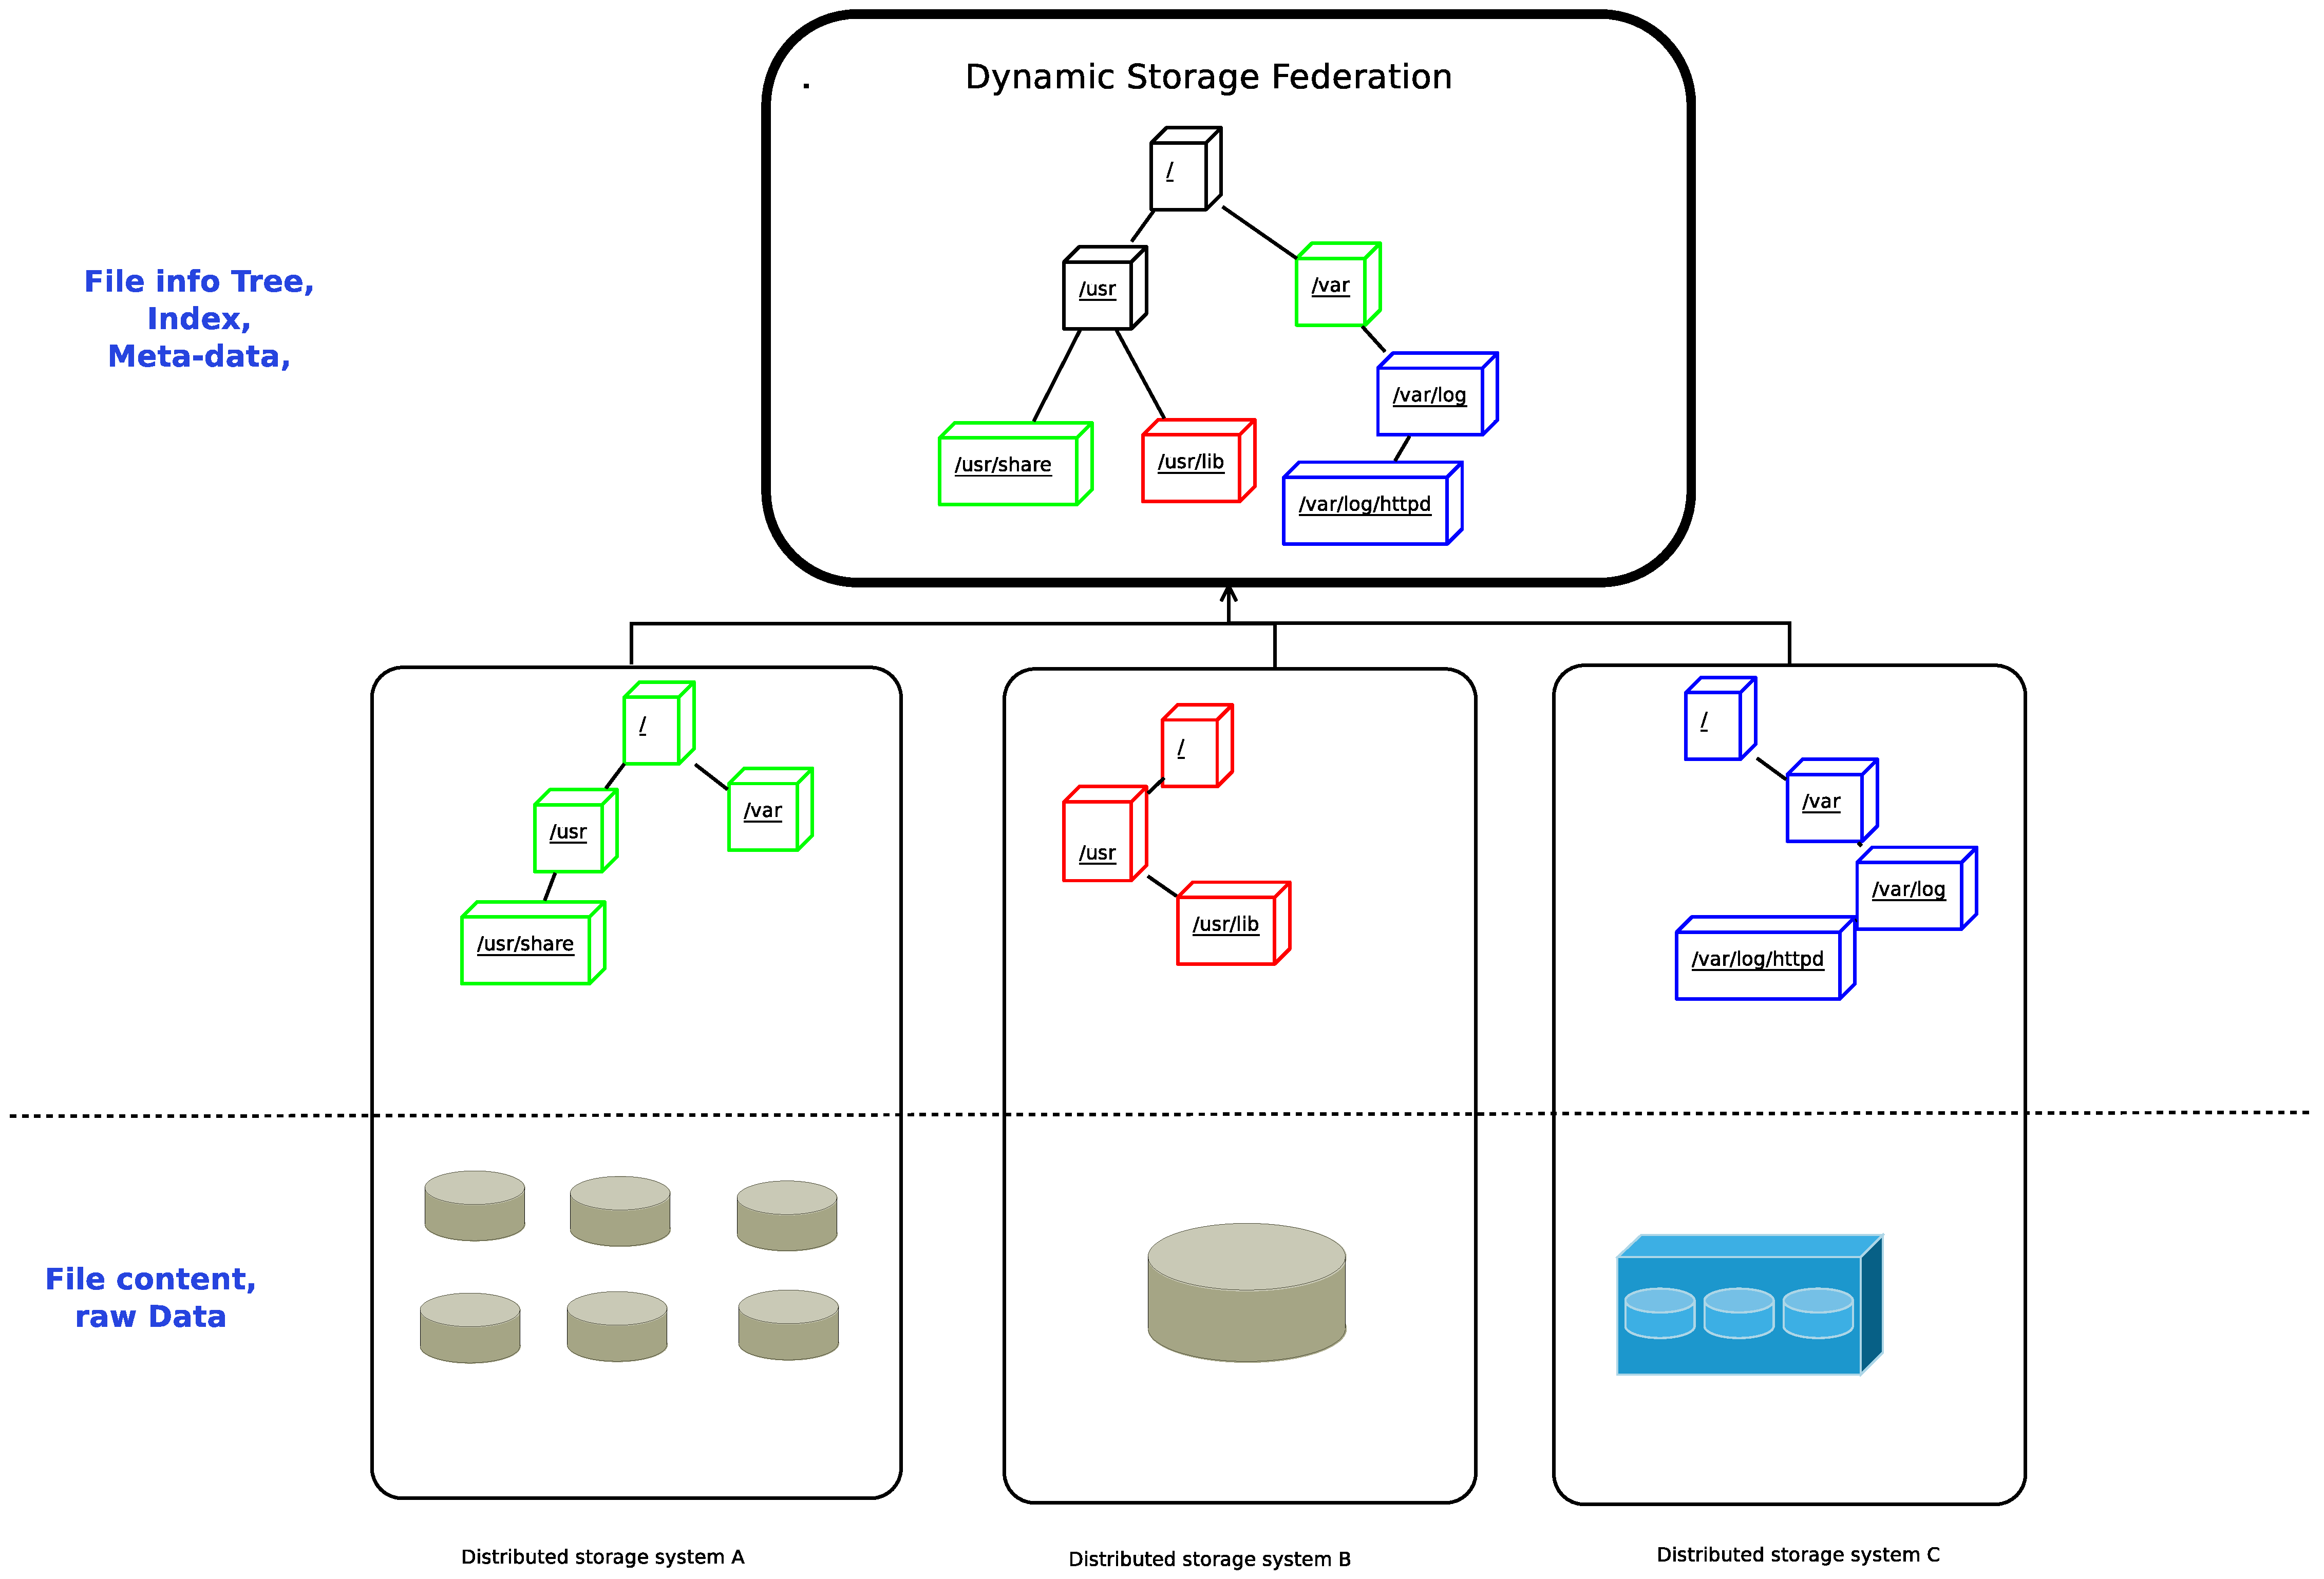
\includegraphics[width=28pc]{diagram-principle.eps}
  \end{center}
  \caption{\label{fig_mergenamespace}How namespaces can be merged to federate three hosts.}
\end{figure}

Figure \ref{fig_mergenamespace} shows an example of the meaning of the term 'Federation' in this context. In the example we have three distributed storage systems, named \textit{A}, \textit{B} and \textit{C}, each one exposing a name space containing files and directories. The upper box in the picture shows how the federated name space looks like. The rule applied is "if a file or directory exists in at least one of the systems A, B or C, then it is considered \textit{as contained in the federated system}".

One more aspect of this aggregation of storage resources is that the aggregating system does not need to keep a persistent index of the content of the systems A+B+C. It can just query the subsystems when any information is needed, and eventually cache in some way the responses it receives.\\

Such a federation of sites has to be intended as a set of storage endpoints (and/or replica location catalogues or name translators) that is:
\begin{itemize}
\item protocol-homogeneous (a client that uses a particular protocol must be able to operate with all the members of the federation, using that protocol)
\item namespace-homogeneous (each file is identified by a unique string key, which we call path/name. If two storage endpoints have a file with the same name, then they are two replicas of the same file.)
\end{itemize}

Given the criteria the WLCG data is distributed through sites, we did not want to limit the design by forcing to create partitions of the data repositories based on the path/name. Although a formally correct idea, it's apparently not compatible with the way LHC data is being distributed and used.\\
 
 In order not to limit the use cases to file fetching, the repositories should support the protocol features that allow an application to analyze data via WAN (with a proper analysis application) \cite{xrdwan}. This is the case of the HTTP and, possibly, nfs4.1 protocols.\\

Although creating several, distinct federations is always possible, the most interesting case is obviously the one for which there is only one big efficient federation, with a logical unique entry point that eventually could be replicated in several places. For the purposes of our project it's immaterial if this big federation aggregates sub-federations or storage endpoints or name translators or replica location catalogues. As a comparison, the xrootd \cite{xrd} federations support this kind of very wide setups by means of a mechanism called \textit{peering}, which has a few constraints. We refer the reader to the xrootd documentation in the case they are not familiar with the concept.\\

The Grid software gives the possibility of choosing among several components the ones that are more suitable for handling the storage and metadata parts of the design of a computing model. Some of them are, for example DPM, LFC, dCache. Nowadays we have also to start considering as parts of the solution the upcoming evolutions of these components \cite{dpmfuture} \cite{dpmnew}, that are headed to supporting standard protocols like HTTP, WebDAV and NFS4.1 in the context of scientific computing. On top of this we must also consider the opportunity of acquiring storage as an external service, as an additional kind of endpoint to fit in a modern design.\\
The goal of the Dynamic Federations project is to give efficient tools that are able to accommodate in a coherent way the variety of storage and metadata endpoints that a distributed, heterogeneous deployment of storage farms will make available. At the same time, the guidelines of the project are to privilege the aspects that are related to performance, scalability and usability of the federation services.


\section{Some use cases}
We describe here a few use cases for our ''storage federation engine'', that we consider as clear examples of the features that our system provides and as deployment use cases that have been tested with the system we designed. These are not intended to be precise specifications of the system. Of course the list is not exhaustive, given the flexibility of the concept. Moreover, the various points do not exclude each other.\\

In the case of a big loosely coupled federation, the choices to redirect a client to a repository or another should be based at least on the availability of the requested resource in that endpoint. Other metrics can be considered, like the geographical location of the client with respect to the various possible servers, and/or the load of the endpoints.
In other words, a client in Switzerland should not be redirected to read data from Taipei, unless the requested data is hosted only in Taipei.\\

We would like to recall that we are treating data access protocols that natively support redirections. The idea is that an application would use only a ''standard'' client (like a Web browser or an application using an HTTP client) to access the data, without additional client-side software layers that emulate the aggregation of the storage centers.

\subsection{DPM and dCache via WebDAV}

Given a number of storage endpoints deploying the WebDAV door of the dCache system, and the upcoming versions of DPM \cite{dpmfuture} \cite{dpmnew}, we wanted to show that a completely transparent federation of them was possible, using the WebDAV protocol.
This use case has been the first one to be demoed by the Dynamic Federations project, and the first two endpoints that were added to a working federation have been a dCache instance at DESY (Germany) and a DPM instance in ASGC (Taipei). The test did what it advertised, i.e. the users could not realize that they were browsing and using a federation of two distant sites. Moreover, the feeling of performance that the system gives is the one of a site that is hosted in the federation's frontend machine, with a fast and smooth interactivity.

\subsection{Add third-party storage farms}

We cite here what was the first formulation of this use case to be fulfilled by the Dynamic Federations project: \\
\textit{We buy from a company a service consisting in 100PB of high performance storage, located in a remote server farm. The company only allows the use of the WebDAV/HTTP protocol to access it, since its technicians do not know anything else, and do not want to internally expose their infrastructure to unknown sophisticated systems, by installing them.\\
We want the clients to be able to see this service through the same entry point that aggregates other similar services in a completely transparent way, at least for the data reading case. We don't want the client applications to be instrumented in order to accommodate this case. We don't want a Data Management system to treat this case as an exception of some kind.\\
This would allow users to browse their files using Internet Explorer without potentially being aware of the location of the items they see, and to run their personal analyses pointing their applications to the unique entry point, using the URLs that they see in the browser.}\\

This use case may also accommodate the use case of the ''Cloud storage providers''. Technically, we chose to use a Cloud storage service provided by T-Mobile (Germany) through WebDAV, which then became a standard component of the various demos of the Dynamic Federations system.

\subsection{Create a small local federation of close sites sharing storage}

Having a flexible system that can manage storage federations opens many possibilities. One of them is being able to create a small federation of sites that share their storage, and appear as a unique storage element. In other words, a common repository (for example an instance of the so-called "conditions data" for a High Energy Physics experiment) may be distributed across collaborating sites. Doing so, the clients would not  need to know the exact location of the file they need, as they would just access it through the federation frontend.

\subsection{Add resources managed by one or more LFCs}

We informally define an \textit{LFC cloud} as a set of storage elements that contain file replicas that are indexed by an instance of an LFC file catalogue. In this example, without loss of generality, we suppose that the content of the LFC is accessible through an HTTP/DAV gateway, like the ones that have been recently released \cite{dpmfuture}.
Let’s suppose that we have two such clouds, as the example fits with no changes also the case in which there are more.\\

A ''storage federation engine'' acts as unique entry point for the two clouds, by hiding the fact that they are two. Hence, an HTTP client would contact the main federations frontend, and will have access to all the metadata from there, because the frontend machine aggregates and caches on the fly the results of the metadata queries that are forwarded to the endpoints.\\
If the client issues an HTTP GET request towards the frontend, this will simply redirect it to one of the endpoints that have just advertised the availability of the requested file.\\ In other words, the client can be redirected to the best endpoint in the most suitable LFC cloud, with a decision based on:
\begin{itemize}
\item availability of the file in the two clouds
\item possibly, proximity of the client with respect to all the available endpoints.
\end{itemize}
The interesting aspect in this example is that no additional indexing of the files is needed to federate the two LFC clouds, and their internal, local workflow can remain untouched. \\
Another worth mentioning point is that also connecting natively to an LFC database is supported by the architecture, as the corresponding plugin is available as well.
We believe that this kind of feature could be beneficial for Virtual Organisations whose content is managed by more than one instance of LFC, in different sites. A worldwide deployment would appear as an unique thing to applications that benefit from having access to the whole repository. At the same time, the local workflows and the ownership of the local catalogues would remain, also avoiding the network latency-related issues that may come from having only one catalogue service for a widely distributed VO.

\subsection{Federating file caches}

The fact that our Dynamic Federations system applies a dynamic behavior to the problem of federating storage and metadata endpoints opens the possibility of federating storage endpoints whose content may change at a faster pace with respect to a regular storage element.
This is the case, for example, of a storage cluster that acts as a file cache, hence files may appear and disappear, depending on the pattern of the file requests that it receives.\\
Such a storage federation that includes caches among its endpoints would have the benefits that come from both concepts:
\begin{itemize}
\item caches would provide their service to the site they belong to, fetching files from elsewhere and keeping them while they are being actively used
\item the same caches would advertise the files that they currently contain to the federation system.
\end{itemize}
The outcome of these two points is that the content of a file cache in a given moment could be used through the federation frontend by some other external client, or, eventually, by some similar file cache system that is trying to fetch the file. As a consequence, the federation frontend would have more endpoints to choose from when asked to redirect a client to a suitable server that hosts a file resource. This aspect, coupled with some other smart endpoint choosing criteria like e.g. geographic proximity, would represent a very relevant feature for a Grid-aware setup.
So far, work is foreseen to verify the usability, in the described context, of the Scalable Proxy Caches \cite{scalableproxycache}.


\subsection{Allow the system to apply geography-aware redirection choices}

A feature that we implemented in our system internally associates geographical coordinates and information to each replica that is known to the federation, by invoking a loadable "Geo" plugin. The same plugin can associate this information to each client request for locating a replica. As a consequence, the system can select the replica that is geographically closer to the client that requested it.\\
An easy implementation of the Geo plugin consisted in wrapping the GeoIP API \cite{geoip}, that seems to provide a more than adequate level of performance (on the order of one million queries per second, as output by its internal tests). The result is that the Dynamic Federation system is able to redirect a client to the replica that is the closest to it, in a very efficient way.


\section{The system}

The Dynamic Federations system is built around a new internal component that was called Uniform Generic Redirector (UGR). The Ugr exposes an API, called \textit{UgrConnector} that gives the functionalities of a namespace, thus including file/replica metadata information and directory listing information.

As visible in Figure \ref{fig_dynafeds1}, the Ugr acts as loader of a set of plugins, which interface it to the external storage and metadata endpoints. Each kind of plugin can talk to a different kind of external endpoint (one or many in principle).\\ Right now we developed the following plugins:

\begin{itemize}
\item A WebDAV/HTTP client plugin, that is able to talk to an external WebDAV/HTTP server endpoint. This plugin is based on an implementation of an advanced wrapper client interface (called DAVIX), built using \textit{libneon} \cite{libneon}. This component supports several kinds of authentication, and supports advanced metadata primitives (e.g. getting file listings with all the metadata information of the items, in a single transaction). 
\item A DMLite-client plugin, that is able to use an instance of DMLite as a source of metadata information. This allows using all the possibilities of integration offered by DMLite, for instance to connect natively to an LFC database or to an HDFS cluster.
\end{itemize}
All the plugins that have been developed so far privilege the internal parallelism, i.e. they are able to perform N tasks in parallel, where N is a parameter that needs to be tuned in order to find the right balance between the overall system performance and the load that can be put towards the endpoints.\\
The set of plugins that are loaded by an Ugr instance (and their configuration) is written in a configuration file. Each plugin can be loaded multiple times, with different parameters and prefix-based filename translations.\\

The typical use of the Ugr is to be loaded by some other frontend system, like for instance the DMLite library \cite{dpmnew}. In this form, Ugr acts as a DMLite plugin, taking full benefit of its architecture and behavior. DMLite is a pluggable, thin software layer that gives abstract functionalities of file catalogue and interface to storage pools. Thanks to its architecture, a very broad range of storage systems can be accessed, through suitable plugins. DMLite can also be plugged into an Apache server, thus accessing all of its features through WebDAV.\\
One of the consequences of this is that, through DMLite, plugging the Ugr into an Apache server becomes easily feasible, as shown in Figure \ref{fig_dynafeds1}.\\

Internally, the Ugr acts as a sophisticated handler of parallel requests for metadata information. The basic behavior on the trigger of a metadata query is as follows:
\begin{itemize}
\item if the query can be satisfied by the local in-memory namespace cache, just use the cache to compute the result. Otherwise:
\item trigger, in parallel, all the plugins by queueing the query into them, then wait for the result.
\item each plugin may internally decompose the query into subqueries (also parallel, depending on the plugin)
\item each plugin acts independently in order to satisfy the query and write its result into the namespace cache
\item when the gathered information is \textbf{sufficient} for that client to get the result, that client only is signalled so that it can get the desired information.
\item the plugins that eventually did not finish the processing just continue, eventually updating the content of the cache with the information they may still gather. 
\end{itemize}

This sequence of actions is performed for any client, in parallel, with no imposed limits to their concurrency inside Ugr.

In the next sections we show sequence diagrams that explain with some more details the internal behavior of such a system, in two relevant cases.

\begin{figure}
\begin{center}
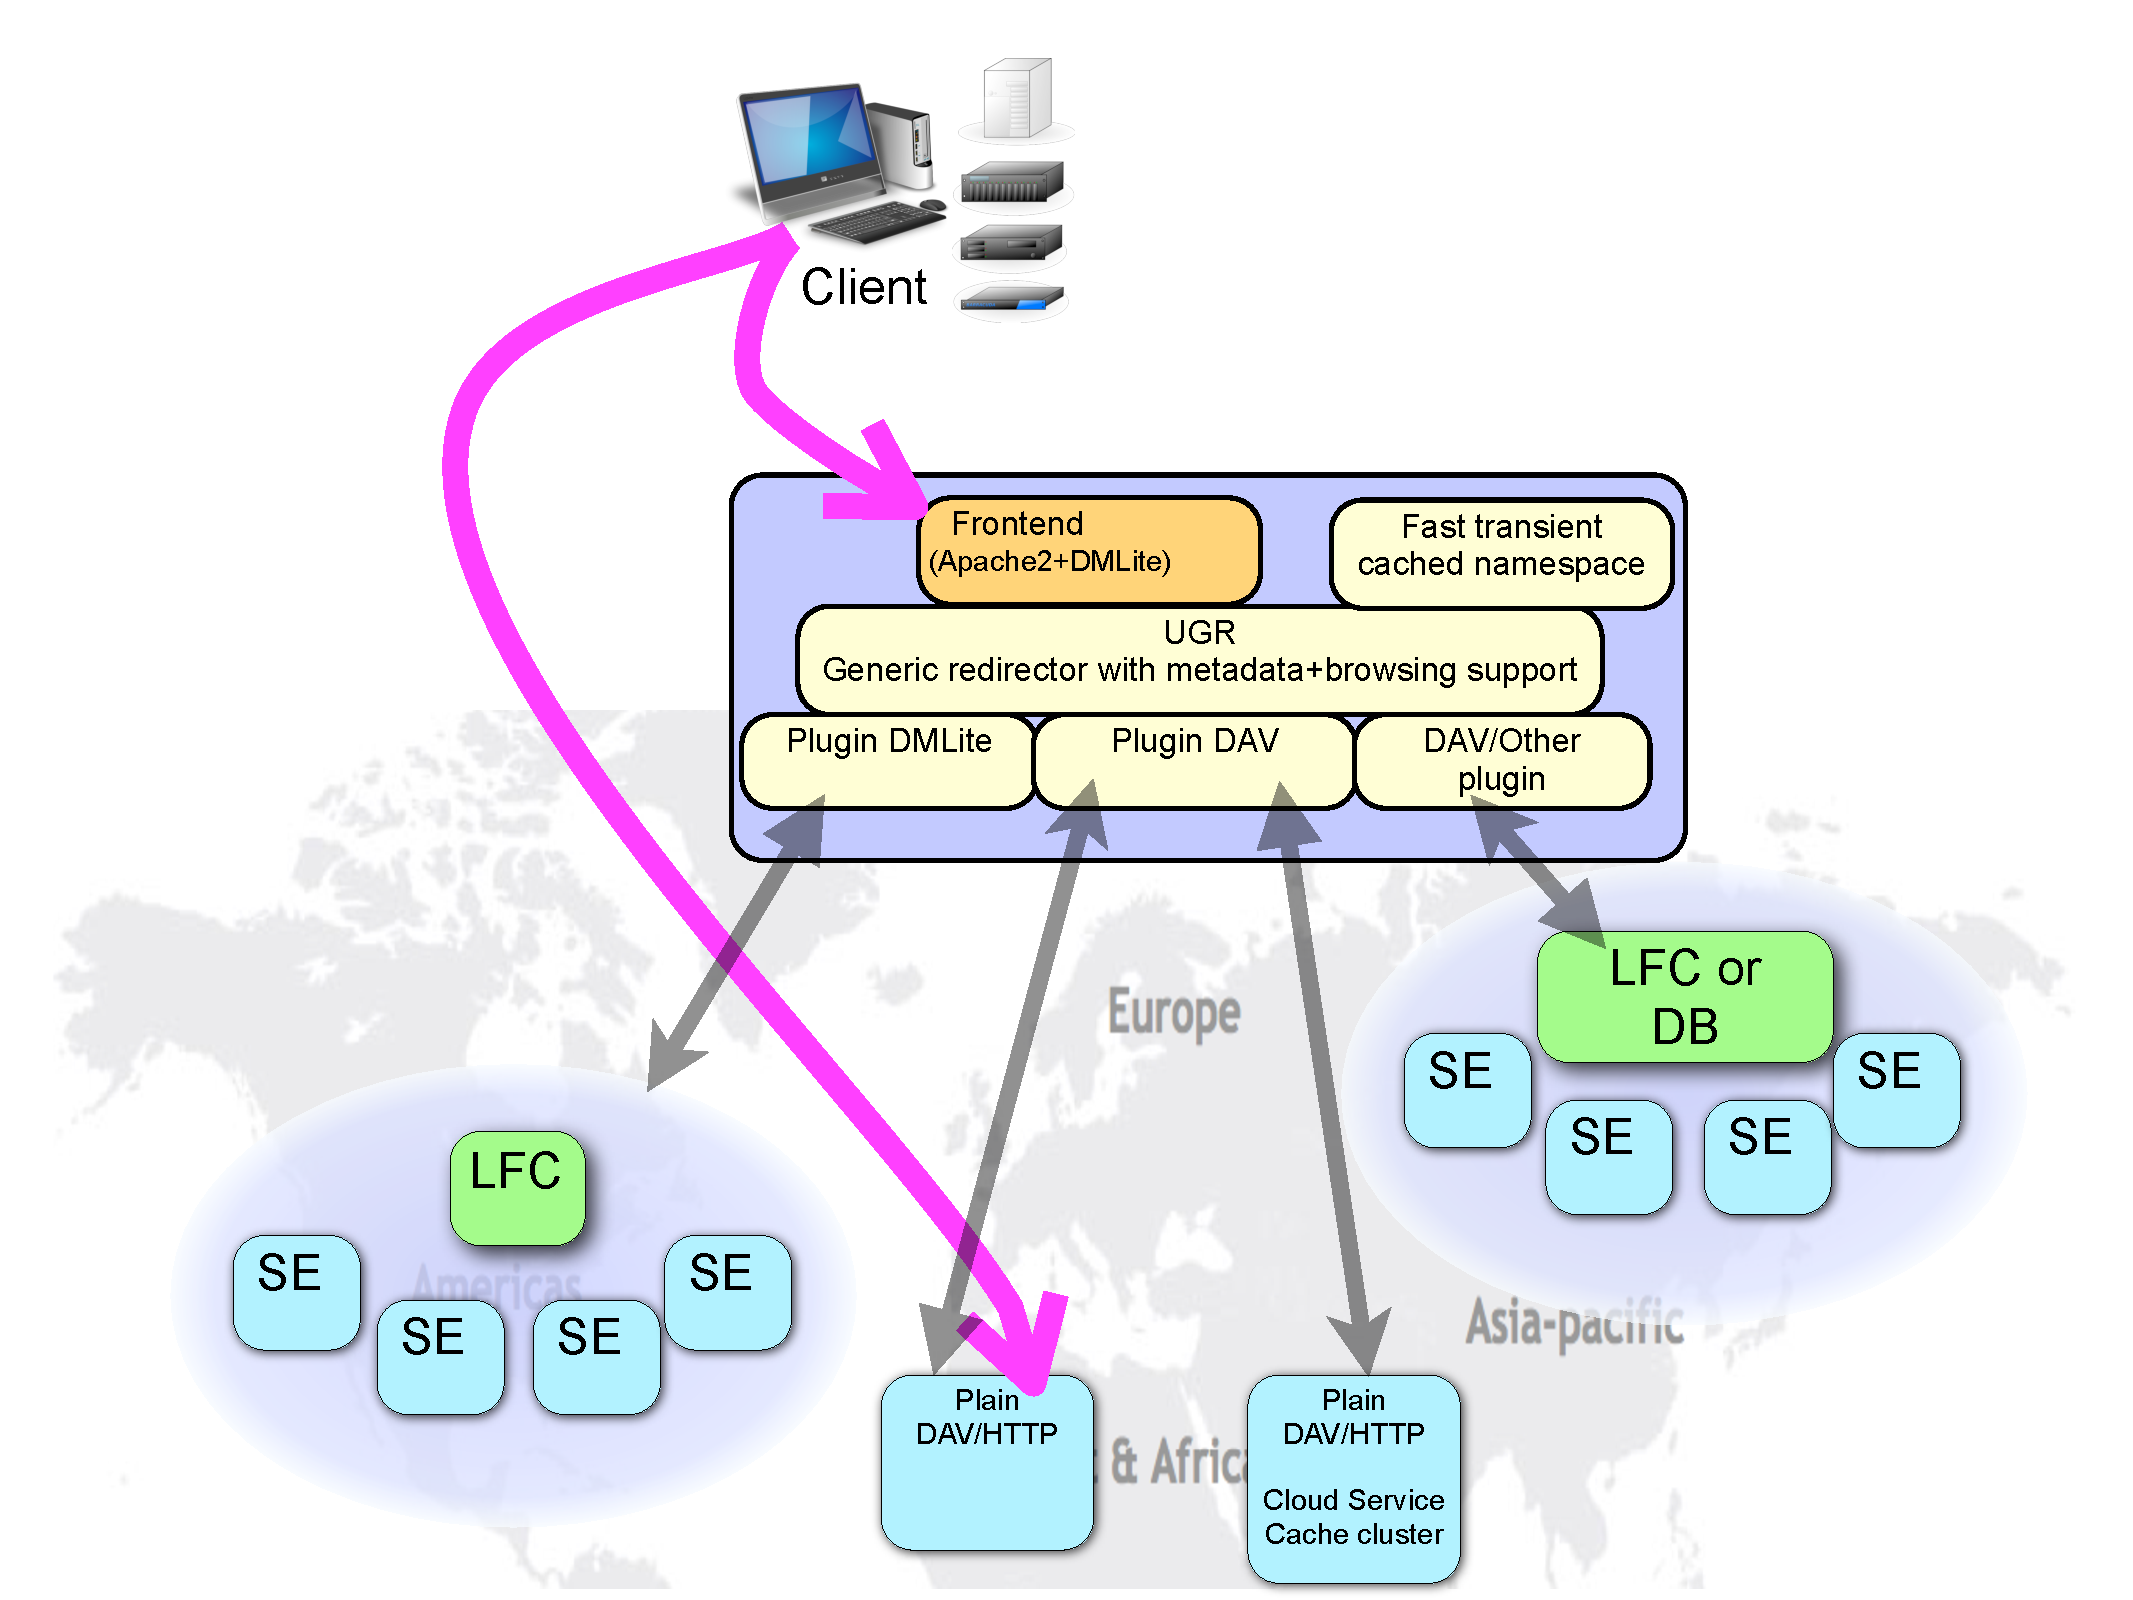
\includegraphics[width=28pc]{dynafeds.eps}
\end{center}
\caption{\label{fig_dynafeds1}Exemplification of the system architecture.}
\end{figure}

\subsection{Two clients issue a stat() request}

In this example, shown in Figure \ref{fig_collab1} two clients want to know some metadata information about file X, e.g. its size. Hence, they invoke the API of the Ugr service and get the response. The response is constructed by the aggregation service on the base of the responses of the various plugins.\\

The clients get the response as soon as the service gets it from the endpoints that it aggregates.
A successive query for the same information gets a cached answer, as shown in the diagram.\\

Any primitive describing this behavior (e.g. getting the size of a file) could give the name to this operation, should the reader be uncomfortable with the choice of \textit{stat} of this example.\\

As previously said, this diagram wants to describe the basic internal interactions of such an aggregator service. The term Client refers here to any system that is able to invoke the API, single or multithreaded. As discussed, in the current deployments this client is an instance of DMLite embedded into an Apache server.

\begin{figure}
\begin{center}
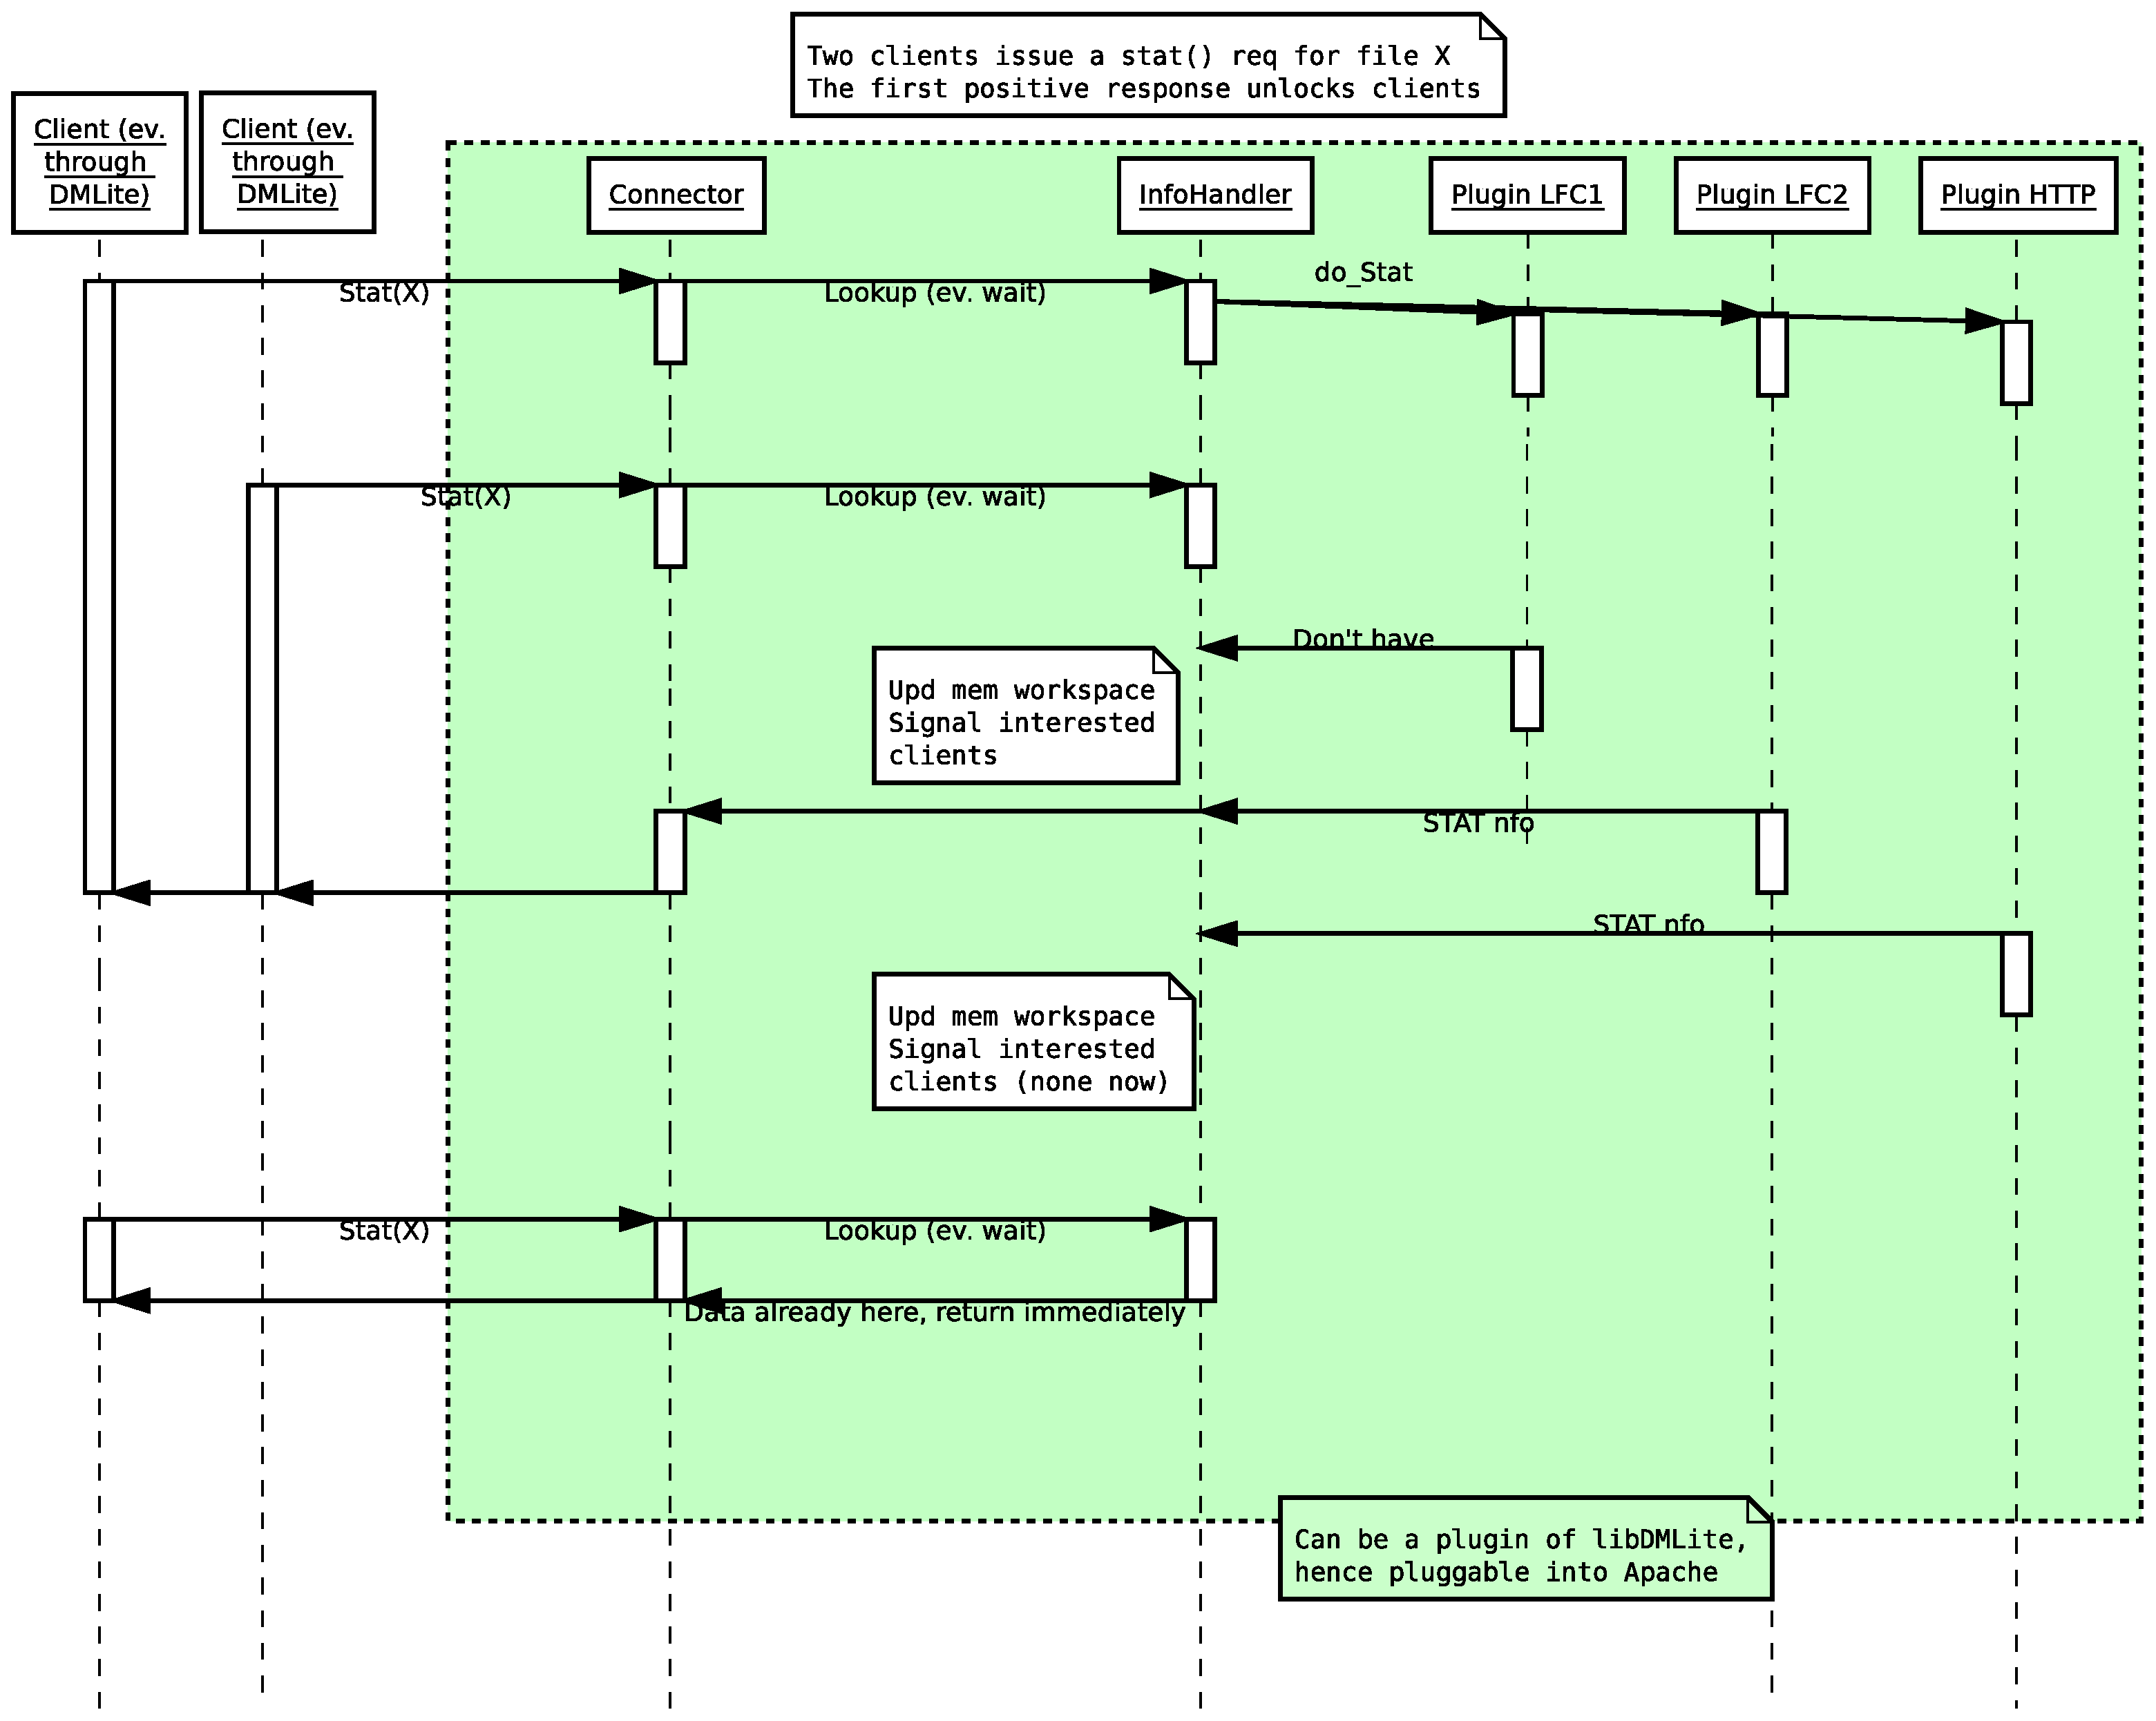
\includegraphics[width=28pc]{collab1.eps}
\end{center}
\caption{\label{fig_collab1}Clients issuing a Stat() request for the same file.}
\end{figure}

\subsection{Two clients request the full list of the replicas of a file}

In this example, shown in Figure \ref{fig_collab1_loc}, two clients want to know the list of the locations of file X, eventually through name translations. Hence, they invoke the API of the Ugr service and get the response. The response is constructed by the aggregation service on the base of the responses of the various plugins.\\

Any primitive with this behavior (e.g. getting a list of replicas) could give the name to this operation, should the reader be uncomfortable with the choice of \textit{locateall} of this example. Some implementations refer to this functionality with \textit{getreplicas}. We wanted to use a different term in order to emphasize the fact that this specification is implementation-agnostic.\\

As previously said, this diagram wants to describe the basic internal interactions of such an aggregator service. The term Client refers here to any system that is able to invoke the API, single or multithreaded. In at least the DPM/LFC deployments this client will likely be an instance of the DMLite library \cite{dpmnew}.\\
 
The difference with respect to the previous case is that in order to discover all the replicas of a file the system has to wait for all the plugins to have finished. In the previous case instead, getting the size of a file just need the answer of the fastest of the endpoints.

 \begin{figure}
\begin{center}
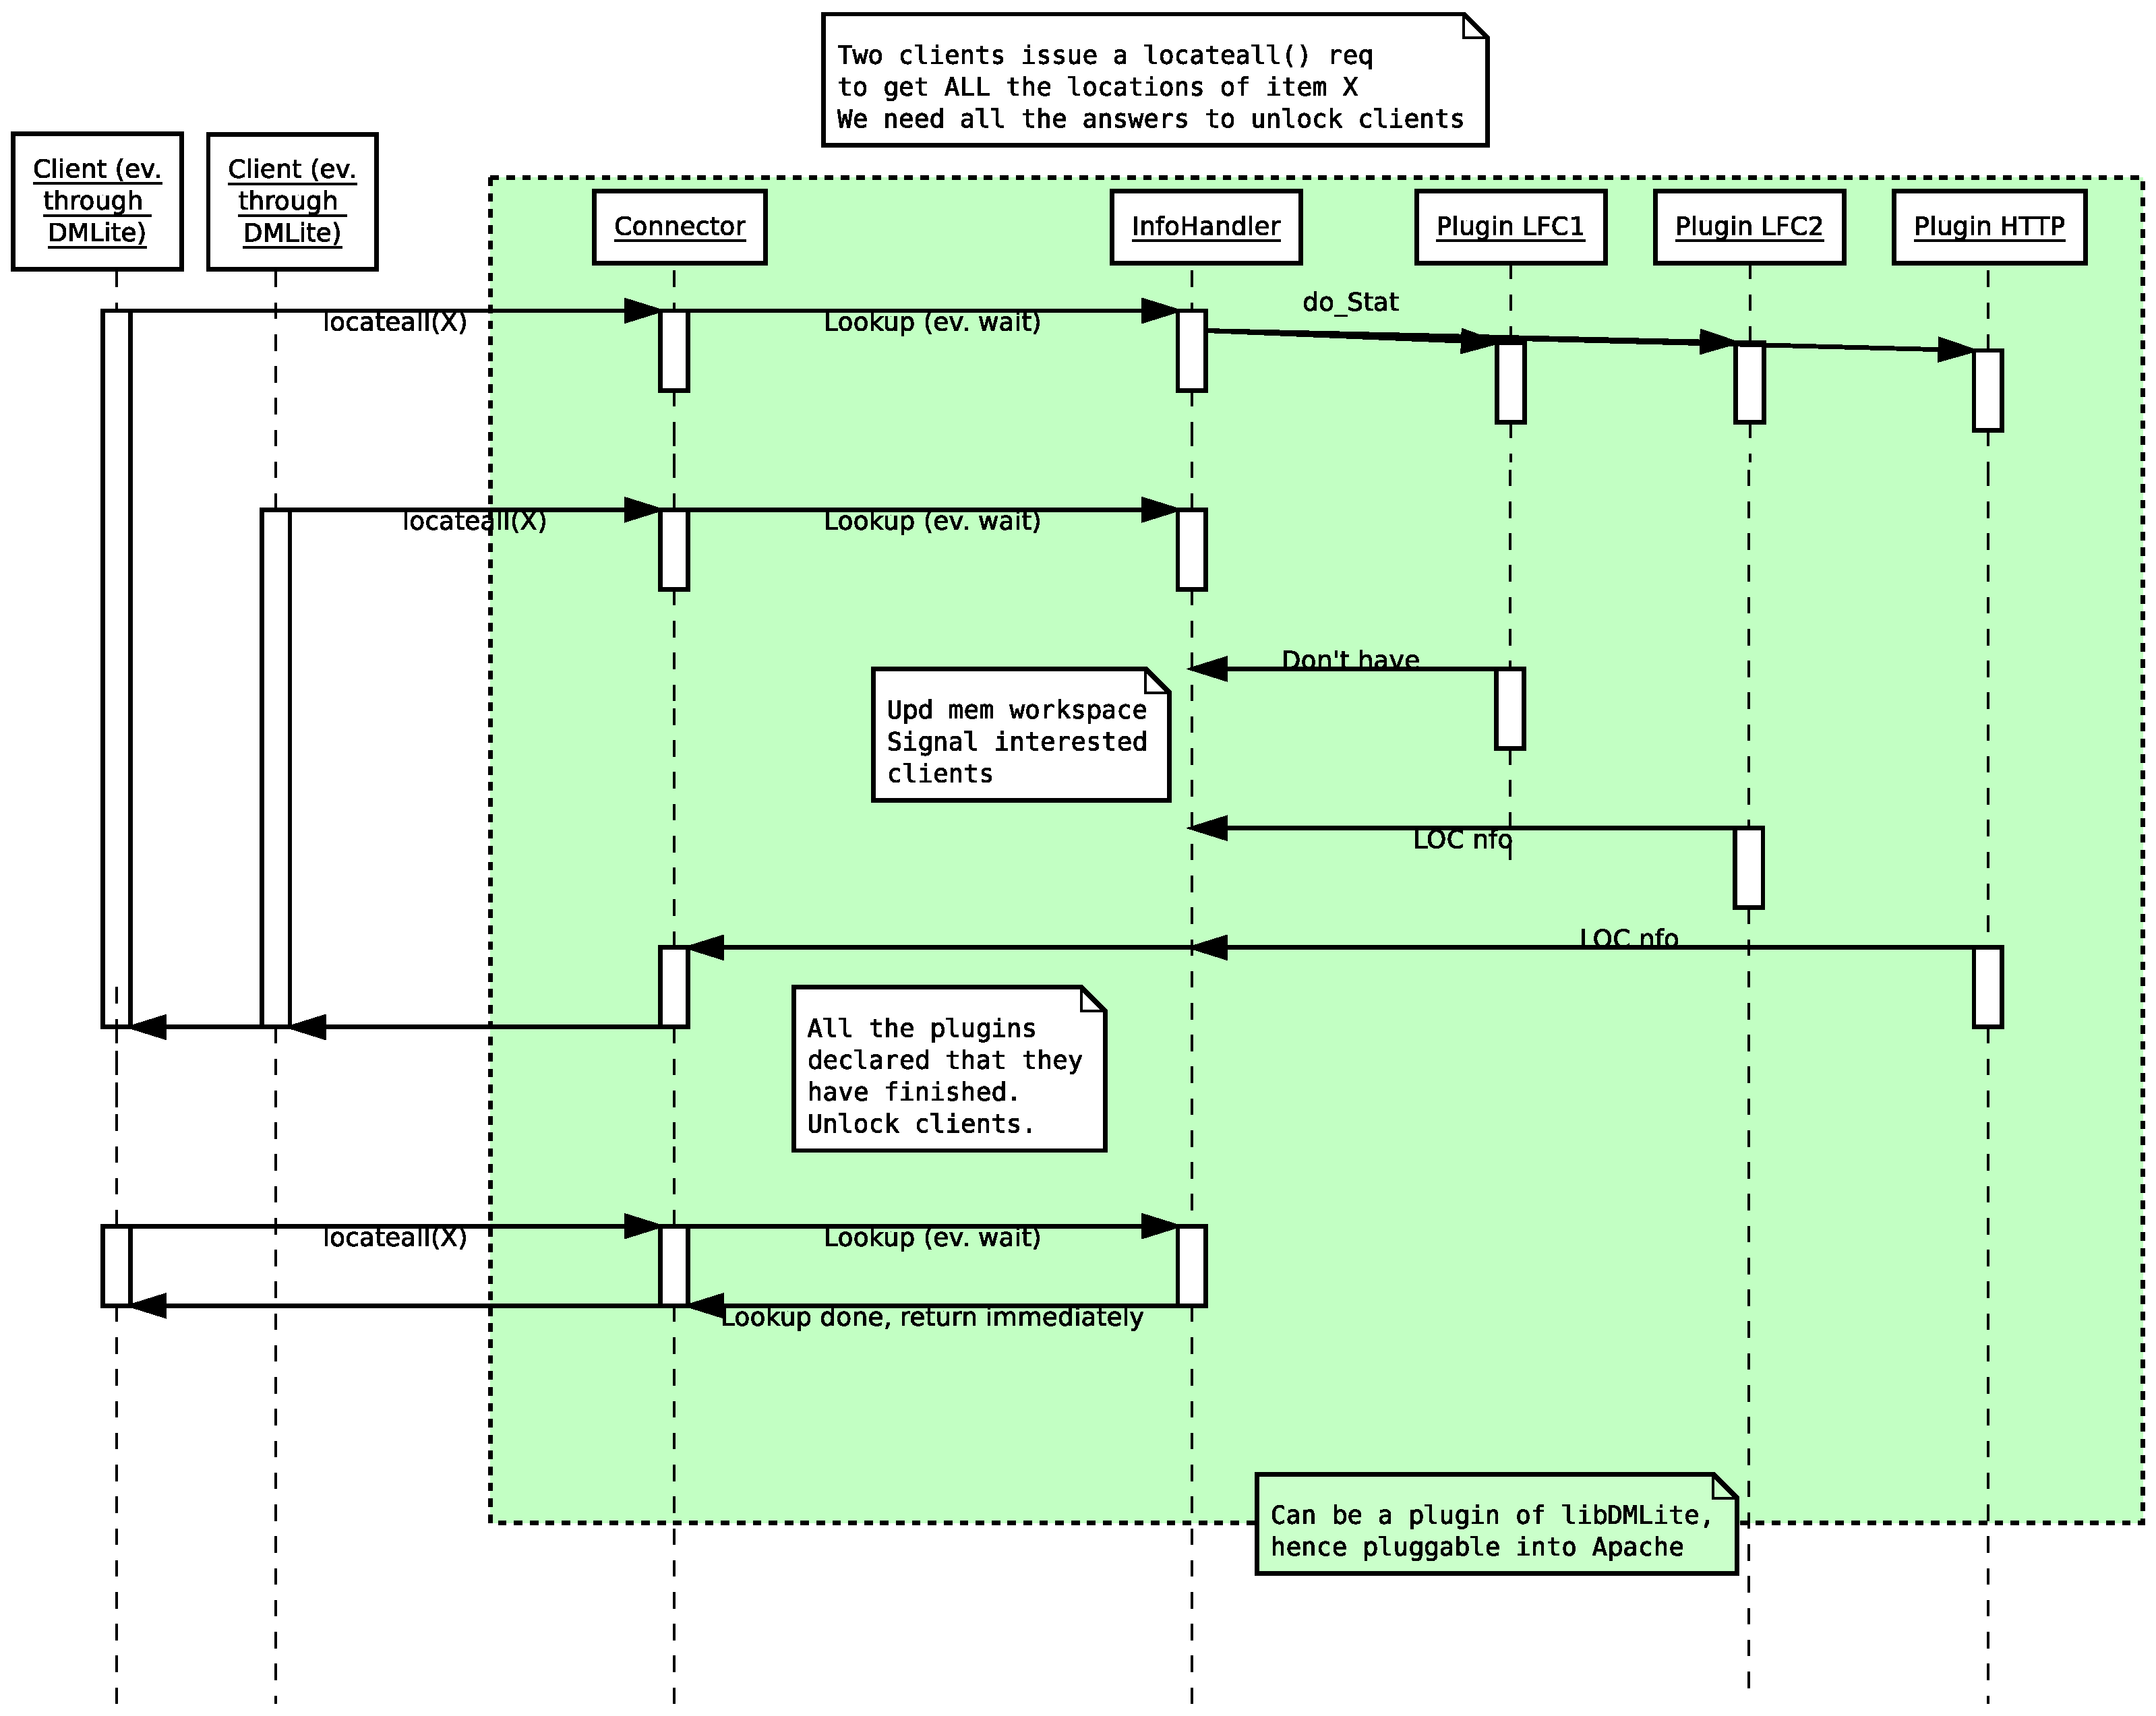
\includegraphics[width=28pc]{collab1_locations.eps}
\end{center}
\caption{\label{fig_collab1_loc}Clients trying to discover all the locations of the same file.}
\end{figure}


\subsection{In-memory volatile namespace and caching}

Figure \ref{fig_cache} shows how the caching structure of UGR works, in order to cache the relevant parts of the federation's namespace.\\

UGR, in the default setup, is treated as a plugin of the Apache srver, hence it is subject to its behaviour, related to multiprocessing and multithreading. Normally, Apache spawns several processes, each one with its own thread pools that serve HTTP requests.\\

Each instance of UGR can do its local computations in a fast local workspace, whose internal behavior is similar to a cache. In order to put in relation the local workspaces of multiple processes, and optimize their behavior, UGR can connect to a memcached service, which must be big enough to cache a significant part of the working set of the storage metadata, i.e. the metadata items that are used more often by the clients.\\

In addition to that, a site hosting the frontend of a large federation may want to deploy more than one machine, under the same DNS name. In this case we may want to deploy a memcached service that is accessed by all the machines in the cluster, like the one shown in Figure \ref{fig_cache}.\\

The simple default configuration installs \textit{memcached} in the same server where Apache and UGR are installed.\\

\begin{figure}
  \begin{center}
    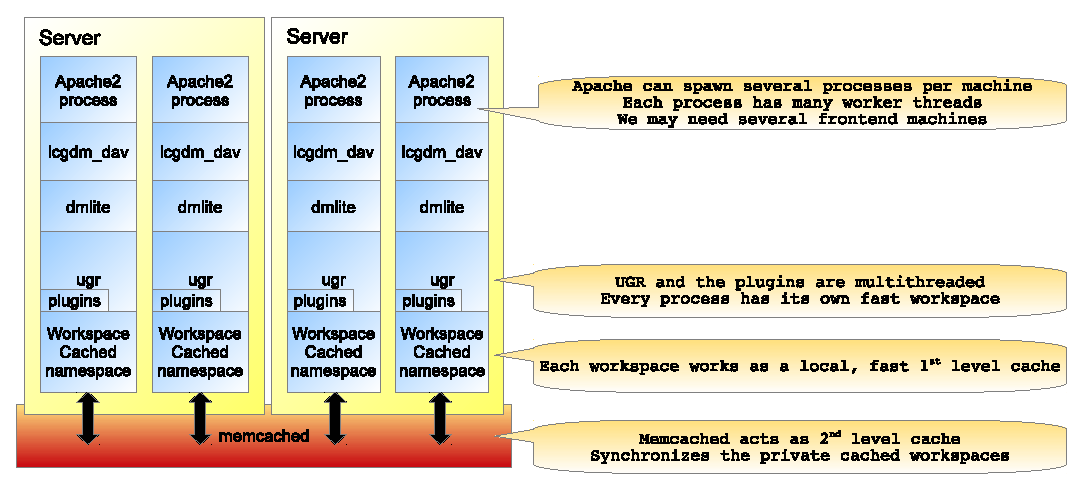
\includegraphics[width=36pc]{cache.eps}
  \end{center}
  \caption{\label{fig_cache}How threads, processes, servers and caches work.}
\end{figure}


\subsection{Simple name translations}

UGR embeds a configurable scheme of name translation, which has the purpose of creating a match between the path prefixes of the resulting global name space and of the individual name spaces of the endpoints whose content is aggregated.\\
The complete scheme is shown in Figure \ref{fig_n2n}. Starting from the left, the clients have the illusion of interacting with a name space that is the federation's namespace, e.g.\\

 \verb"/myfed/dteam/mydir/myfile"\\
 
 which (in the case of a setup with HTTP) may come from an URL like:\\
 
 \verb"http://<host>/myfed/dteam/mydir/myfile" .\\\
 
 Then, internally, if the path starts with the prefix specified in \textit{n2n\_pfx}, this prefix is stripped from the path and the \textit{n2n\_newpfx} is put in its place.
 
 The resulting path/filename is what is handled by the internal workspace, and propagated to the plugins.
 
  The plugin themselves can implement their own prefix-based name translation, which appends a prefix before contacting their endpoint.\\
  
 Setting up the name translations in order to minimize the length of the filenames in the internal workspace is a very good idea.\\





\begin{figure}
  \begin{center}
    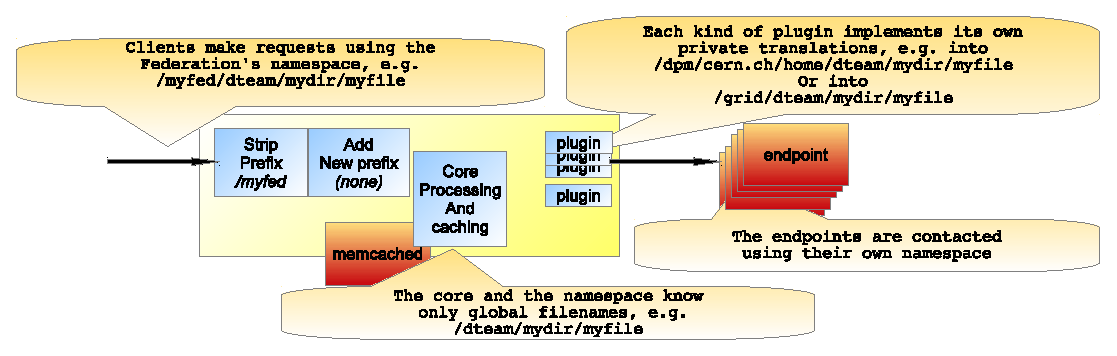
\includegraphics[width=36pc]{n2n.eps}
  \end{center}
  \caption{\label{fig_n2n}How the default name translations work in order to federate storage metadata endpoints.}
\end{figure}

\section{Typical deployment of a Dynamic Federations frontend}

UGR is a very generic component that can be used in a variety of ways that are agnostic of the communication protocol that is used to talk to the clients. By \textit{typical deployment} we mean a description of the default configuration that comes when installing it from the official packages.\\
In this case, UGR is used to create storage federations based on the HTTP/WebDAV protocols, using Apache2 as frontend, and the DMLite library both as an adaptor between Apache and UGR, and as an optional way to aggregate other external metadata sources (like site-local instances of DPM and LFC).\\
Figure \ref{fig_fullconfig} shows how the default deployment of an UGR frontend looks like:

\begin{itemize}

	\item Apache2 is the frontend to the clients;
	\subitem \textit{/etc/ugr/zlcgdm-ugr-dav.conf} is the file that defines the virtual server that is fed through lcgdm\_dav and DMLite;
	\item lcgdm\_dav is the Apache module that is able to talk to DMLite, and to use it as a source of information;
	\item DMLite is a pluggable layer that provides storage element functionalities;
	\subitem \textit{/etc/ugr/ugrdmlite.conf} is a DMLite configuration file, which loads UGR as a source of metadata.
	\item UGR is loaded as DMLite plugin that provides name space information;
	\subitem \textit{/etc/ugr.conf} is the file that configures UGR.
	\item UGR has its internal high performance buffer caches, and is more efficient with an external memcached instance that synchronizes their content, acting as a 2nd level cache.
	\item The loaded plugins have their own configuration parameters. In the case of the HTTP/DAV plugin, the parameters are set in the same Ugr configuration file.
	
\end{itemize}

\begin{figure}
  \begin{center}
    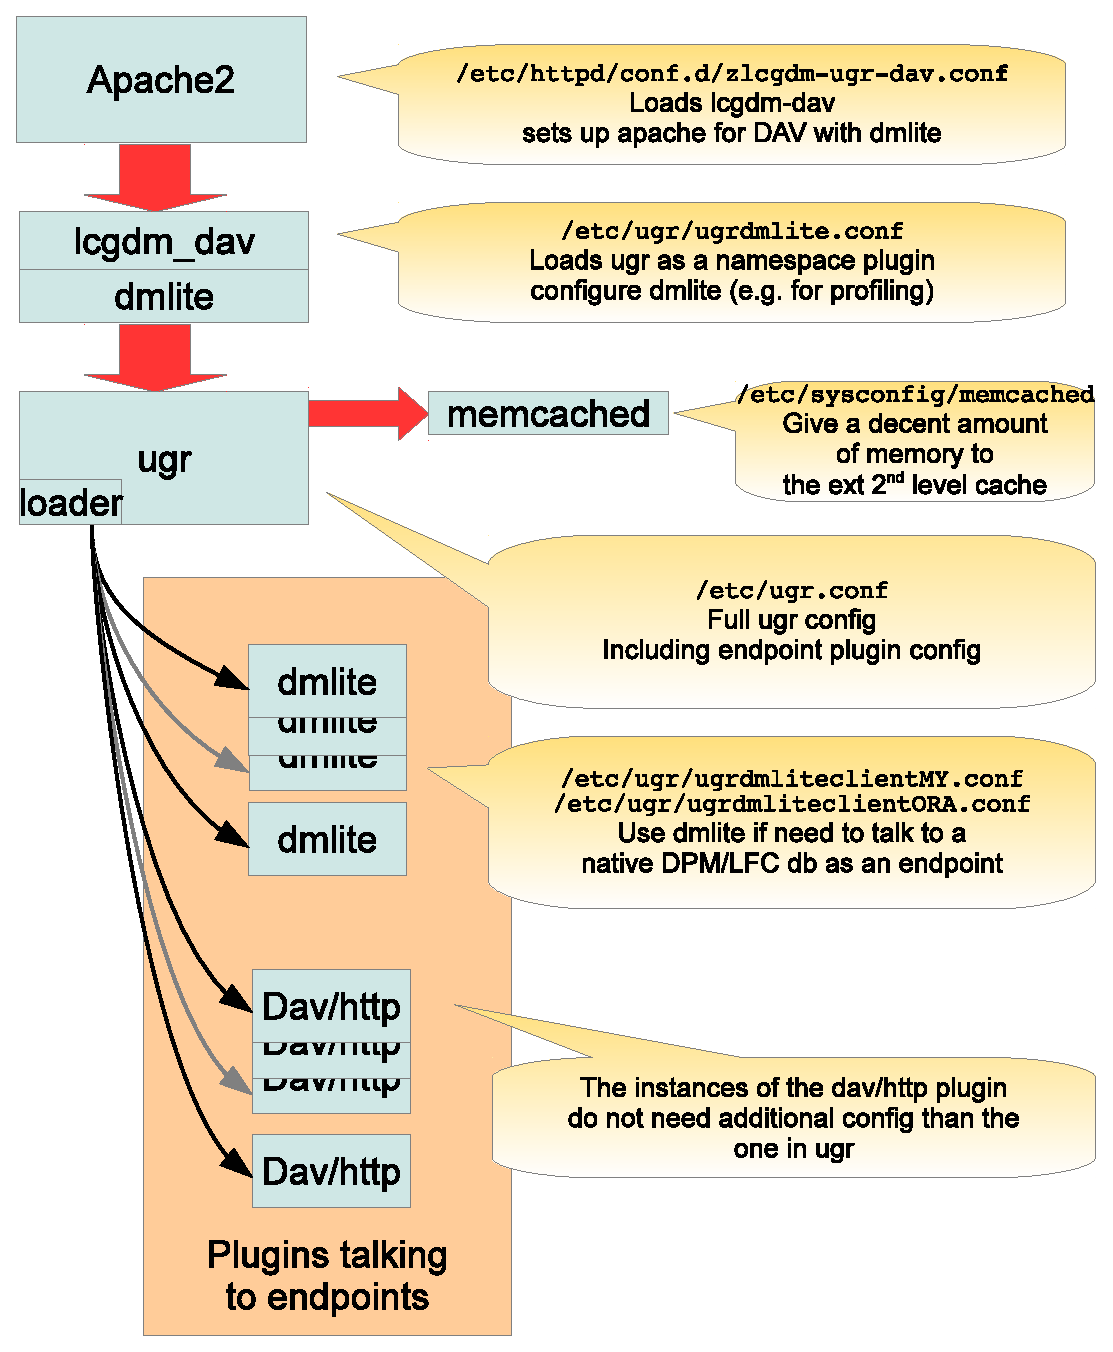
\includegraphics[width=30pc]{fullconfig.eps}
  \end{center}
  \caption{\label{fig_fullconfig}Configuration structure of the typical deployment.}
\end{figure}

\section{Configuration parameters reference}
In this section, we document the UGR configuration directives and their usage. In the default deployment, these directives are contained in the \textit{/etc/ugr.conf} configuration file.

\subsection{Ugr core configuration}

\subsubsection{glb.debug}

 Sets the UGR log verbosity.\\
 
 Syntax:\\

\verb"glb.debug: <level>"\\

\verb"<level>" is the desired debug level, from 0 to 10.\\ \\
 NOTE: UGR internally uses \verb"syslog" to log its activity, in the \verb"user" class. We refer to the \verb"syslog" documentation for the platform in use in order to configure its behavior, e.g. to output the log to a logfile.\\
 
  NOTE: a debug level higher than 1 severely affects the performance of UGR. Never set it to a value higher than 1 in a production server.\\

\subsubsection{\label{glb.locplugin}glb.locplugin}

 Load an UGR location plugin. This directive can be specified many times, thus loading several plugins.\\
 
 Syntax:\\

\verb"glb.locplugin[]: <path/name.so> <ID> <max_concurrency> [parameters]"\\

where:

\begin{itemize}
\item \verb"<path/name.so>" is the full path to the shared library that implements the plugin
\item \verb"<ID>" is a unique name that is given to this plugin instance. This is used to identify it in this configuration file, and give settings that are private to that loaded instance. These other settings have the syntax:\\
      \verb"glb.locplugin.<ID>.<parm>: <value>"\\
     where <parm> is the plugin-specific parameter that we want to set.
\item \verb"<max_concurrency>" is the maximum number of threads that can enter the plugin at the same time
\item \verb"[parameters]" is a plugin-specific series of space-limited parameters
\end{itemize}


\subsubsection{glb.waittimeout}

The maximum time in seconds that a client can wait for some information to be collected by UGR. This is just a guard time. If reached, some external endpoint may be overloaded or not responsive. In this case, UGR may decide to internally treat it as disabled, until it becomes responsive again.
\\
Syntax:\\
\verb"glb.waittimeout: <number>"

Default value: 180

\subsubsection{glb.maxlistitems}
Mark as non listable any directory that contains more than a certain number of items. This avoids thrashing the cache in difficult situations. This setting deals only with listing, not with the metadata of the individual files or subdirectories that are needed by the clients. In other words, the items in the directory are always accessible, no matter how many they are.\\
Syntax:\\
\verb"glb.maxlistitems: <number>"


Default value: 10000



\subsection{Global name translation}

UGR can process the file paths it is requested, in order to normalize them by means of prefix substitutions. The typical case is to internally remove the prefix that is instead present in the requests.

\subsubsection{glb.n2n\_pfx}

Remove the given prefix, if found in the requested URL.\\
Syntax:\\
\verb"glb.n2n_pfx: <string_prefix>"

Default value: none
\\
Example:\\

\verb"glb.n2n_pfx: /myfed"

If the requested path starts with \verb"/myfed", remove this prefix, so that internally in UGR that file is known without prefix.

If the user requests /myfed/atlas/fabrizio/testfile.txt, internally the file will be known as /atlas/fabrizio/testfile.txt
 
\subsubsection{glb.n2n\_newpfx}

After having eventually stripped out a prefix with the \verb"n2n_pfx" directive, replace it with a new prefix.\\
Syntax:\\
\verb"glb.n2n_pfx: <string_prefix>"

Default value: none




\subsection{Infohandler advanced parameters}
The infohandler parameters influence how the internal UGR buffers collect  and reconstruct the information that comes from the endpoints, and act as a fast in-memory first level cache.



\subsubsection{infohandler.maxitems}
Set the maximum number of items in the cache.\\
Syntax:\\
\verb"infohandler.maxitems: <number>"\\

Default value: 1000

\subsubsection{infohandler.itemttl}
Set the maximum time (in seconds) an item is allowed to stay in the cache after it has been referenced.\\
Syntax:\\
\verb"infohandler.maxttl: <number>"\\
Default value: 600



\subsubsection{infohandler.itemmaxttl}
Set the maximum time (in seconds) an item is ever allowed to stay in the cache (even if it was referenced in the meantime).\\
Syntax:\\
\verb"infohandler.itemmaxttl: <number>"\\
Default value: 3600


\subsubsection{infohandler.itemttl\_negative}
Set the maximum time (in seconds) a negative information (like a "file not found" error) is allowed to stay in the cache.
Syntax:\\
\verb"infohandler.itemttl: <number>"\\
Default value: 10


\subsubsection{infohandler.useextcache}
If true, instantiate a 2nd level cache that uses \textit{memcached}. This cache will be shared among all the processes that are spawned.\\
Syntax:\\
\verb"infohandler.useextcache: <true|false>"\\
Default value: true

\subsection{extcache.memcached.server[]}
In the case the \verb"infohandler.useextcache" is set to true, UGR will try to contact an external \textit{memcached} cluster.  This section describes the parameters that configure that.\\

 Syntax:\\

\verb"extcache.memcached.server[]: <IP_address>[:port]"\\

Add one memcached server to contact. Multiple entries like this add multiple servers to contact, in order to support advanced memcached clustering configurations.\\

Default value: 127.0.0.1:11211

\subsubsection{extcache.memcached.ttl}
Set the maximum time (in seconds) an item is allowed to live in the external memcached.
Syntax:\\
\verb"extcache.memcached.ttl: <number>"\\
Default value: 43200\\

\subsubsection{extcache.memcached.useBinaryProtocol}
Enable/disable the memcached binary protocol.
Syntax:\\
\verb"extcache.memcached.useBinaryProtocol: <true|false>"\\
Default value: true\\

\subsection{DAV plugin}

The DAV plugin, when loaded as a location plugin instance, points to an external DAV or HTTP endpoint, to consider its content as part of the storage federation.\\

Syntax:\\
\verb"glb.locplugin[]: /usr/lib64/ugr/libugrlocplugin_dav.so <ID> <concurrency> <URL prefix>"

The parameters \verb"<ID> <concurrency>" have already been described in the section \ref{glb.locplugin}

The parameter \verb"URL prefix" is the URL prefix that points to the endpoint to be federated. Both \verb"http://" and \verb"https://" are supported. Please note that if a prefix of the files stored in the external storage has to be ignored, then it has to be added to this \verb"URL prefix". \\

A typical example of this is the following:\\
\verb"dav_plugin_dcache_desy 30 http://sligo.desy.de:2880/pnfs/desy.de/data"\\ \\

where the prefix \verb"/pnfs/desy.de/data" has to be stripped in order to consider the files as belonging to a uniform name space.\\

In other words, a file named:\\
\verb"/pnfs/desy.de/data/atlas/fabrizio/testfile.txt"\\

will be known to UGR as\\
\verb"/atlas/fabrizio/testfile.txt"\\

The DAV plugin has several parameters that configure the way it works and authenticates with the servers. For all these parameters, \verb"<ID>" is the name that was assigned to the specific plugin instance we want to refer to.

\subsubsection{glb.locplugin.$<$ID$>$.ssl\_check}
Enable or disable the SSL validity check of the remote host.\\
Syntax:\\
\verb"glb.locplugin.<ID>.ssl_check: <true|false>"\\
Default value: true\\
\subsubsection{glb.locplugin.$<$ID$>$.cli\_certificate}
Path to a local file containing the client side credentials to use when contacting this endpoint. Only the p12 format is supported.\\
Syntax:\\
\verb"glb.locplugin.<ID>.cli_certificate: <path/file>"\\
Default value: none\\
\subsubsection{glb.locplugin.$<$ID$>$.conn\_timeout}
TCP connection timeout (in seconds) to use when establishing a connection to this endpoint. \\
Syntax:\\
\verb"glb.locplugin.<ID>.conn_timeout: <timeout>"\\
Default value: 5\\
\subsubsection{glb.locplugin.$<$ID$>$.ops\_timeout}
TCP communication timeout (in seconds) to use when sending/receiving data from this endpoint.\\
Syntax:\\
\verb"glb.locplugin.<ID>.ops_timeout: <timeout>"\\
Default value: 60\\
\subsubsection{glb.locplugin.$<$ID$>$.status\_checking}
Enable or disable the asynchronous endpoint status checker. If enabled, the endpoint will be probed at regular intervals of time.\\
Syntax:\\
\verb"glb.locplugin.<ID>.status_checking: <true|false>"\\
Default value: true\\
\subsubsection{glb.locplugin.$<$ID$>$.status\_checker\_frequency}
Set the frequency (in milliseconds) of the status checker.\\
Syntax:\\
\verb"glb.locplugin.<ID>.status_checker_frequency: <time>"\\
Default value: 10000\\
\subsubsection{glb.locplugin.$<$ID$>$.auth\_login}
Set the username to use in the case of endpoints that support user/pasword login.\\
Syntax:\\
\verb"glb.locplugin.<ID>.auth_login: <username>"\\
Default value: none\\
\subsubsection{glb.locplugin.$<$ID$>$.auth\_passwd}
Set the password to use in the case of endpoints that support user/password login.\\
Syntax:\\
\verb"glb.locplugin.<ID>.auth_passwd: <password>"\\
Default value: none\\



\subsection{DMLite client plugin}

The DMLite client plugin, when loaded as a location plugin instance, instantiates a DMLite instance as a source of metadata information to federate. The typical usage is to contact natively an LFC or DPM database, for increased performance.\\

Syntax:\\
\verb"glb.locplugin[]: /usr/lib64/ugr/libugrlocplugin_dmliteclient.so <ID> <concurrency> <config>"

The parameters \verb"<ID> <concurrency>" have already been described in the section \ref{glb.locplugin}

The parameter \verb"<config>" is the full path to a DMLite configuration file. To configure DMLite, we refer to the DMLite documentation.

\subsubsection{locplugin.$<$ID$>$.xlatepfx}
Sets up the path/name translation that the DMLite plugin can apply, in order to match the namespace of the endpoint to the federation's namespace.

Syntax:\\
\verb"locplugin.<ID>.xlatepfx: <internal_workspace_prefix> <prefix_to_strip>"

\verb"<internal_workspace_prefix>" is the prefix that is kept in the internal UGR workspace. It is generally \verb"/".\\
\verb"<prefix_to_strip>" is the prefix that has to be stripped from the namespace of the endpoint, to make it match with the federation's namespace.\\

Example:\\

\verb"locplugin.mydpmdb.xlatepfx: / /dpm/cern.ch/home"\\

This example serves to federate a DPM database. A file named in DPM \verb"/dpm/cern.ch/home/atlas/fabrizio/testfile.txt" would be known as \\
\verb"/atlas/fabrizio/testfile.txt" in the internal UGR workspaces.

\section*{Acknowledgment}

This work was partially funded by the EMI project under European
Commission Grant Agreement INFSO-RI-261611



\begin{thebibliography}{9}

\bibitem{ibmglamour} IBM Glamour \verb"http://www.almaden.ibm.com/storagesystems/projects/glamour/". 


\bibitem{rfc5716} RFC 5716
\verb"http://tools.ietf.org/html/rfc5716"


\bibitem{gluster} Gluster
\verb"http://gluster.com"

\bibitem{glusterwiki} Gluster on Wikipedia
\verb"http://en.wikipedia.org/wiki/GlusterFS"


\bibitem{fedfs} FedFS
\verb"http://discolab.rutgers.edu/fs/"

\bibitem{xrdwan} Scalla/xrootd WAN globalization tools: Where we are
Fabrizio Furano and Andrew Hanushevsky 2010 J. Phys.: Conf. Ser. 219 072005
\verb"http://iopscience.iop.org/1742-6596/219/7/072005/"

\bibitem{xrd} The xrootd.org homepage
\verb"http://www.xrootd.org"

\bibitem{datamgmthep}
Furano F. Data Management in HEP: an approach. 
The European Physical Journal Plus
Volume 126, Number 1 (2011), 12, DOI: 10.1140/epjp/i2011-11012-2

\bibitem{dpmnew}Web enabled data management with DPM \& LFC
Alejandro Alvarez Ayllon, Alexandre Beche, Fabrizio Furano, Martin Hellmich, Oliver Keeble and Ricardo Brito Da Rocha
CHEP2012

\bibitem{dpmfuture}DPM: Future Proof Storage
Alejandro Alvarez, Alexandre Beche, Fabrizio Furano, Martin Hellmich, Oliver Keeble, Ricardo Rocha
CHEP2012

\bibitem{dpmcomp} DPM components
\verb"https://svnweb.cern.ch/trac/lcgdm/wiki/Dpm/Dev/Components"

\bibitem{geoip}
"This product includes GeoLite data created by MaxMind, available from http://www.maxmind.com/."

\bibitem{scalableproxycache}
Cristian Traian Cirstea
Grid Data Access: Proxy Caches and User Views
Eindhoven University of Technology
Stan Ackermans Institute / Software Technology
ISBN 978-90-444-1067-9


\bibitem{libneon}
\verb"http://www.webdav.org/neon/"

\end{thebibliography}


\emph{DRAFT}\\

\emph{DRAFT}\\

\emph{DRAFT}\\

\emph{DRAFT}\\

\emph{DRAFT}\\

\emph{DRAFT}\\

\emph{DRAFT}\\

\emph{DRAFT}\\

\emph{DRAFT}\\


\end{document}